% Chapter 2

\chapter{Conception et Développement} % Chapter title

\label{ch:2} % For referencing the chapter elsewhere, use \autoref{ch:3} 

De prime abord, il est important de souligner que la création d'un \ac{llm} est un processus coûteux et exigeant en termes de données. Les modèles de langage existants, tels que GPT-4 \cite{openai2023gpt4}, ont été développés avec une quantité massive de données et une puissance de calcul considérable. Cependant, pour adapter ces modèles au contexte juridique congolais, il serait peu pratique, voire impossible, de construire un \ac{llm} à partir de zéro en raison de contraintes de ressources.

Inspiré par Heydar Soudani \cite{soudani2024fine}, notre approche consiste à utiliser un modèle de langage existant comme point de départ (voir Table~\ref{table:llm-models}). En prenant un modèle pré-entraîné, nous pouvons bénéficier des connaissances et des capacités linguistiques déjà intégrées dans le modèle. Nous chercherons ensuite à affiner ce modèle pré-entraîné pour le rendre spécifique au système juridique congolais. Pour ce faire, nous utiliserons deux méthodes principales : le \ac{ft} et le \ac{rag}.

\paragraph{\acf{ft}} \hspace{0pt}

Le \ac{ft} implique de prendre un modèle de langage pré-entraîné, tel que GPT-4, et de le spécialiser pour le domaine spécifique du système juridique Congolais. Cette méthode consiste à ajuster les poids du modèle en le nourrissant avec des données spécifiques au contexte juridique Congolais. En utilisant des corpus de textes juridiques, des décisions de justice et d'autres ressources pertinentes, nous entraînerons le modèle à comprendre et à générer des réponses cohérentes et précises aux questions juridiques \cite{yue2023disclawllm}.

\paragraph{\acf{rag}} \hspace{0pt}

En parallèle, nous utiliserons également l'approche du \ac{rag}, qui combine la génération de texte avec des techniques de recherche d'informations. Le \ac{rag} permet au chatbot d'accéder à une base de connaissances juridiques étendue et de récupérer des informations pertinentes en réponse aux requêtes des utilisateurs. En utilisant des index de recherche efficaces et des algorithmes de récupération d'informations, le chatbot peut fournir des réponses bien informées en s'appuyant sur une grande variété de sources \cite{lewis2021retrievalaugmented}.

En définitive, La conception et le développement présentés dans ce mémoire s'articulent autour de deux axes principaux. D'une part, nous nous concentrerons sur le modèle \ac{llm}, en suivant toutes les étapes de conception et de développement détaillées dans la section \ref{ch:1:section:ml-process}. Ce processus englobe la collecte initiale des données brutes jusqu'au déploiement final du modèle sélectionné dans un environnement de production. D'autre part, l'attention sera également portée sur le développement du chatbot, qui agit en tant qu'application web. Cette interface utilisateur servira de pont pour accéder au modèle \ac{llm}, facilitant ainsi l'interaction entre les utilisateurs et le système juridique Congolais à travers le chatbot. 

Ce dernier ne représente pas seulement un outil d'accès, mais aussi une manière intuitive et efficace de mettre en application les capacités du modèle \ac{llm}, permettant aux utilisateurs d'obtenir des réponses et des informations juridiques pertinentes de manière interactive.

\section{Les données}

Compte tenu de nos contraintes et objectifs (voir Section~\ref{ch:0:section:limitaions}), les données n'ont pas besoin d'être structurées selon un format particulier, à condition qu'elles soient disponibles sous forme textuelle. Cette flexibilité permet d'exploiter une large variété de sources d'information juridique sans nécessiter de processus de prétraitement complexe pour adapter les données à un format spécifique.

Notre jeu de données sera principalement constitué de documents juridiques provenant de diverses sources officielles et spécialisées, afin d'englober une vaste étendue de la législation et de la doctrine juridique congolaise.

Il est à noter que, bien que les données ne requièrent pas un format spécifique, leur qualité textuelle est essentielle. Cela implique un travail de vérification pour s'assurer de la fiabilité, de la pertinence et de l'actualité des informations collectées. Ce processus permettra de minimiser les erreurs et les ambiguïtés dans les réponses fournies par le chatbot, assurant ainsi une assistance juridique de qualité aux utilisateurs.

\subsection{Les sources d'informations}

\begin{table}[h]
\centering
\begin{tabular}{|l|p{10cm}|}
    \hline
    \textbf{Source} & \textbf{Description} \\
    \hline
    Journal Officiel & Publications officielles qui contiennent les nouvelles lois, décrets, et annonces légales, offrant une source à jour des évolutions législatives. \\
    \hline
    Lois et Décrets & Textes législatifs et réglementaires qui forment la base du système juridique congolais, essentiels pour comprendre le cadre légal en vigueur. \\
    \hline
    Jurisprudences & Décisions de justice issues des tribunaux, fournissant des exemples concrets d’application des lois et des interprétations juridiques. \\
    \hline
    Articles d’Actualité Juridique & Articles publiés par des spécialistes et des médias juridiques, offrant des analyses et des commentaires sur les évolutions récentes du droit et les cas d’intérêt. \\
    \hline
    Commentaires de Juristes & Contributions d’experts dans le domaine juridique, y compris des analyses détaillées, des critiques, et des interprétations de divers aspects du droit. \\
    \hline
\end{tabular}
\caption{Sources d'information dans le système juridique Congolais}
\label{table:sources-legales-congo}
\end{table}

La numérisation et l'adoption croissante d'Internet en République Démocratique du Congo (RDC) ont considérablement facilité l'accès aux documents légaux officiels. Désormais, un nombre croissant de ces documents est accessible librement en ligne, offrant une opportunité sans précédent pour la recherche et l'analyse juridique. Des plateformes telles que Leganet.cd \footnote{\href{https://leganet.cd}{https://leganet.cd}} jouent un rôle crucial dans l'agrégation et la diffusion de ces documents, constituant ainsi une ressource inestimable pour les praticiens du droit, les chercheurs, et le grand public intéressé par le droit congolais.

Dans le cadre de notre effort pour enrichir notre modèle avec une base de données complète et à jour sur le droit congolais, nous envisageons d'explorer ces diverses sources en ligne. L'objectif est de collecter un large éventail de documents, allant des textes législatifs et réglementaires aux décisions de justice et aux analyses d'experts, afin de capturer l'étendue et la profondeur du cadre juridique congolais. Cette démarche vise non seulement à fournir à notre modèle une richesse de connaissances et de perspectives sur le droit congolais mais aussi à garantir que les réponses générées soient à la fois informées et pertinentes, reflétant fidèlement les principes et les pratiques juridiques actuels.

Pour faciliter la découverte et l'exploration de ces ressources en ligne, nous envisageons d'utiliser l'\acs{api} Google Custom Search \footnote{\href{https://developers.google.com/custom-search/v1/introduction}{https://developers.google.com/custom-search/v1/introduction}}. Cet outil nous permettra d'automatiser la recherche et de visualiser rapidement les résultats, identifiant ainsi les sites les plus pertinents et fiables où les documents juridiques Congolais sont disponibles. Cette approche automatisée nous aidera à optimiser le processus de collecte de données, en assurant une couverture des sources d'information juridique pertinentes pour notre modèle.

\newpage
\paragraph{Les mots clés} \hspace{0pt}

Les mots-clés jouent un rôle crucial dans le processus de recherche, particulièrement lorsqu'il s'agit de collecter des données spécifiques à un domaine tel que le Droit Congolais. Ils servent de fondement pour affiner les requêtes de recherche et accéder efficacement à l'information pertinente.

\begin{listing}[!ht]
\begin{minted}{python}
keywords = [
    "Constitution", "civil", "Code pénal",
    "Code de travail", "Code foncier ", "Jurisprudence",
    "Droits humains", "Justice transitionnelle", "Droit minier",
    "l'environnement", "commercial", "sociétés",
    "Propriété intellectuelle", "famille", "Violence sexuelle et droit",
    "international humanitaire", "Institutions judiciaires congolaises", 
    "Réforme judiciaire",
    "Lutte contre la corruption", "affaires", "Arbitrage et médiation",
    "bancaire et financier congolais", "fiscal congolais", 
    "Contrats et obligations en congolais",
    "assurances", "santé", "l'éducation",
    "technologies de l'information", "humanitaire",
    "Participation politique et droit"
]
\end{minted}
\caption{Liste des mots clés à utiliser pour la recherche.}
\label{appendix:code:python:search-keywords}
\end{listing}

Cette liste englobe une gamme étendue de domaines juridiques, allant du cadre constitutionnel et législatif général à des domaines plus spécifiques tels que le droit minier, le droit fiscal, et le droit des affaires. Elle inclut également des aspects liés à la jurisprudence, aux publications officielles, et aux analyses d'experts.

Après avoir établi notre liste de mots-clés, nous pouvons créer une fonction qui interagit avec l'\acs{api} Google Search. Cette fonction se sert de la bibliothèque \textbf{Requests} \footnote{\href{https://pypi.org/project/requests/}{https://pypi.org/project/requests/}} pour lancer une requête GET vers l'\acs{url} de l'\acs{api}, en incorporant les paramètres que nous avons spécifiés. Les données renvoyées par l'\acs{api} nous parviennent sous forme de \acs{json}.

\begin{listing}[!ht]
\begin{minted}{python}
params = {
  'q': query,
  'orTerms': ' '.join(keywords).lower(),
  'start': start,
  'key': "xxxxxxxxxxxxxxxxxxxxxxxxxxxxxxxx",
  'cx': 'xxxxxxxxxxxxxxxxxxxx',
  'lr': 'lang_fr',
  'fileType': 'pdf',
  'num': 10
}
\end{minted}
\caption{Dictionnaire des paramètres utile à l'utilisation de l'\acs{api} Google Custom Search}
\label{appendix:code:python:search-google-params}
\end{listing}

Le dictionnaire \textbf{params} contient plusieurs paramètres configurés pour la requête de recherche, des explications détaillées sur l'utilisation des paramètres sont disponible sur la documentation \footnote{\href{https://developers.google.com/custom-search/v1/reference/rest/v1/cse/list}{https://developers.google.com/custom-search/v1/reference/rest/v1/cse/list}} :

\textbf{q}: Le terme principal de la recherche. \\
\textbf{orTerms}: Une chaîne de caractères contenant tous les mots-clés joints par un espace, servant à élargir la recherche à ces termes connexes. \\
\textbf{fileType}: Restreint les résultats aux fichiers d'un type spécifique, ici des PDF. \\
\textbf{lr} : Limite la recherche aux documents dans la langue spécifiée, ici le français. \\
\textbf{num}: Détermine le nombre de résultats de recherche à retourner, ici 10 résultats.

La fonction est conçue pour récupérer les résultats d'une seule page à la fois. Pour explorer un ensemble plus large de résultats, nous allons nous appuyer sur la constante \textbf{MAX PAGES}. En procédant à une itération, nous collecterons les résultats de plusieurs pages jusqu'à atteindre la limite fixée par \textbf{MAX PAGES}.

\begin{listing}[!ht]
\begin{minted}{python}
import requests
import json
import pickle

MAX_PAGES = 10

def search(start=1):
    url = 'https://www.googleapis.com/customsearch/v1'
    query = 'droit congolais'
    response = requests.get(url, params=params)
    return response.json()

try:
    websites = []
    for page in range(1, MAX_PAGES + 1):
        next_page = ((page - 1) * 10) + 1
        results = search(next_page)
        websites.extend(results.get("items", []))

    with open('data.pickle', 'wb') as f:
        pickle.dump(websites, f)
except Exception as e:
    raise e
\end{minted}
\caption{Fonction de recherche via l'\acs{api} Google Custom Search}
\label{appendix:code:python:search-google-function}
\end{listing}

Après avoir recueilli les résultats, nous exploitons la bibliothèque \textbf{Pandas} \footnote{\href{https://pandas.pydata.org/}{https://pandas.pydata.org/}}, qui facilite à la fois la visualisation des données et leur enregistrement dans un fichier au format \acs{csv}.

\begin{listing}[!ht]
\begin{minted}{python}
import pandas as pd 

rows = []
for item in websites:
    row = {
        'Title': item.get('title'),
        'Link': item.get('link'),
        'Snippet': item.get('snippet')
    }
    rows.append(row)

df = pd.DataFrame(rows)
df.head(100)
\end{minted}
\caption{Visualisation et exportation avec Pandas}
\label{appendix:code:python:search-google-visualization}
\end{listing}


\begin{figure}[H]
    \centering
    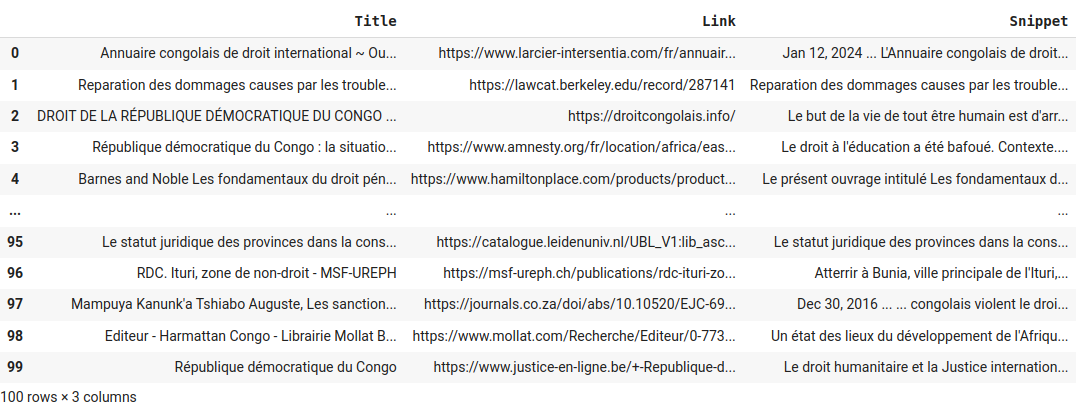
\includegraphics[width=15cm]{gfx/fig-google-search-result.png}
    \caption{Résultat de la recherche via L'\acs{api} Google Custom Search}
    \label{fig:google-search-result}
\end{figure}

\newpage
\newpage
\subsection{Collecte des données}
\subsection{Création du Dataset}
\subsection{Pré-traitement et Formalisations des données}
\subsection{Stockage des données}

\section{Adaption du LLM avec l'approche RAG}
\subsection{Pré-traitement et Création des Embeddings}
\subsection{Construction de l'index de recherche}
\subsection{Fonction de distance vectorielle}
\subsection{Requêtes sur l'index de recherche}
\subsection{Déploiement de l'index de recherche}

\section{Adaption du LLM avec l'approche Fine-tuning}
\subsection{Pré-traitement et Formalisation}
\subsection{Création du modèle}
\subsection{Déploiement du modèle}

\section{Conception de l'application Web}
\subsection{Modélisation de la base de données}
\subsection{Architecture et choix technologique}
\subsection{Diagrammes UML}
\subsection{Développement}

\section{Déploiement et mis en production}
